
\subsection{Pipe model}\label{se:pipe_model}
In this subsection a model for a pressurized pipe will be elaborated. 
%To calculate the flow from the valve, seen in figure \ref{fig:block_diagram_system_overview}, the pressure losses in the Mickey Mouse setup must be known. This section will establish the equation for calculating the pressure loss across a pipe. 

In figure \ref{fig:pipe_3d} an illustration of a pressurized pipe is shown.
\begin{figure}[H]
\centering
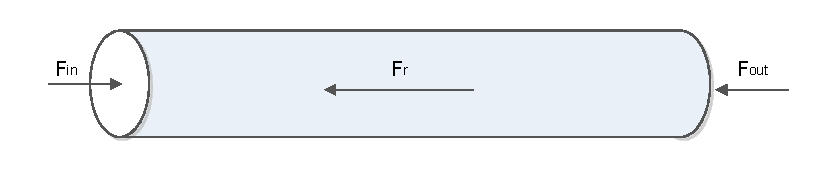
\includegraphics[width=0.9\textwidth]{report/modeling/pictures/pipe_3d.pdf}
\caption{Illustrate the forces within a pipe.}
\label{fig:pipe_3d}
\end{figure}


A model for a pipe is derivate from Newton second law. Where the three forces shown in figure \ref{fig:pipe_3d}, $F_{in}$, $F_r$ and $F_{out}$. $F_{in}$ is the force going into the pipe, $F_r$ is the resistance force within the pipe, such as pipe wall and bends. And lastly $F_{out}$ which is the force going out of the pipe. 
%The derivation of the pipe model is based on figure \ref{fig:pipe_3d}, the pipe model is made, with three different forces, $F_{in}$ which is the pressure force going into the pipe, $F_r$ which is the resistance force in the pipe also known as drag force and lastly $F_{out}$ which represents the pressure force pushing to the left.

Newton's second law applied for the pipe, 
\begin{equation}\label{eq:pipe_newton}
m\cdot \frac{d}{dt}v = F_{in} - F_{out} - F_r 
\end{equation}

Where $m$ is the mass of the water $[kg]$, $v$ is the velocity of the water $\left[\frac{m}{s}\right]$ and the resultant forces $F_{in}$, $F_r$ and $F_{out}$ $[N]$.  

The mass of the water can be written as density times the volume of the pipe,

\begin{equation}
m = \rho \cdot V 
\end{equation}

Where $\rho$ is the density of liquid $\left[\frac{kg}{m^3}\right]$ and $V$ the volume of the pipe $\left[m^3\right]$.


%The equation \ref{eq:pipe_newton} is expressing that the water mass multiplied with the water acceleration is equal to the resultant force.\\
%The mass of the water can be expressed as: 
%\begin{equation}
%m = \rho \cdot V \enhed{kg}
%\end{equation}
%Where:\\
%$\rho$ is the density of the water. $\enhed{kg/m^3}$\\
%$V$ is the volume of the pipe. $\enhed{m^3}$\\

Assuming the pipe is a cylinder, with a constant cross-sectional area along the pipe, the volume of the pipe can be written as, 
\begin{equation}
 V=A \cdot l
\end{equation}
Where A is the area of a circle $[m^2]$ and $l$ is the length of the pipe [m].
%$A$ is the area of a circle. $\enhed{m^2}$\\
%$l$ is the pipe length. $\enhed{m}$\\

Inserting the previous expressions in equation \ref{eq:pipe_newton} the following is obtained,
\begin{equation} \label{eq:pipe_newton_2}
\rho \cdot A \cdot l \cdot \frac{d}{dt}v = F_{in}-F_{out}-F_r 
\end{equation}

The velocity of the water is written as,
\begin{equation}
v=\frac{Q}{A} 
\end{equation}

Where $Q$ is the flow through the pipeline $\left[\frac{m^3}{s}\right]$.

The input, output and resistance force are written as $F=p \cdot A$, where $p$ is the pressure [Pa]. Inserting the expression in \ref{eq:pipe_newton_2} the following is obtained,
\begin{equation}
\rho \cdot A \cdot l \cdot \frac{d}{dt}\left(\frac{Q}{A}\right) = p_{in}\cdot A - p_{out}\cdot A - p_r \cdot A 
\end{equation}

Simplified to,
\begin{equation}\label{eq:pipe_w_pr}
\frac{\rho \cdot l}{A}\cdot \frac{d}{dt}Q = \Delta p - p_r
\end{equation}
Where the pressure difference is expressed as $\Delta p$ and the area is divided on both sides.

The resistance pressure can now be divided into two resistance, namely form resistance and surface resistance \cite{swamee_pipe}. 

\textbf{Surface resistance:}\\
The surface resistance describes the pressure loss across a straight pipe.
\begin{equation}\label{eq:surface_resistance}
h_f=\frac{8\cdot f\cdot l}{\pi^2\cdot g\cdot d^5} \cdot |Q|\cdot Q
\end{equation}
Where $h_f$ is the head loss for the surface resistance of the pipe $[m]$, $f$ is a coefficient for surface resistance, also knows as the friction factor, $g$ is the gravitational acceleration $\left[\frac{m}{s^2}\right]$ and $d$ is the diameter of a circular pipe $[m]$.

\textbf{Form resistance:}\\
The form resistance describes the pressure losses from fittings in a hydraulic network, 
\begin{equation} \label{eq:form_resistance}
h_l=k_L \frac{ |v|\cdot v }{2\cdot g}
\end{equation}
Where $h_l$ is the head loss for the form resistance of the pipe [m] and $k_L$ is the form-loss coefficient.

The form-loss coefficient varies for different components e.g. threaded elbows and tees. The coefficient for the different components can be found in \cite{fundamentals_of_fluid_mechanics}. 

The pressure resistance in the pipe is expressed as:
\begin{equation}\label{eq:pr_resistance}
p_r=\rho \cdot g \cdot h 
\end{equation}

By substituting $p_r$ in equation \ref{eq:pipe_w_pr} with equation \ref{eq:pr_resistance} the following is obtained,

\begin{equation} \label{eq:pipe_sub_pr}
\frac{\rho \cdot l}{A}\cdot \frac{d}{dt}Q = \Delta p - \rho \cdot g \cdot h 
\end{equation}

The surface and form, equations \ref{eq:surface_resistance} and \ref{eq:form_resistance}, can be inserted into equation \ref{eq:pipe_sub_pr},

% \begin{equation} \label{eq:pipe_sub_pr_2}
% \frac{\rho \cdot l}{A}\cdot \frac{d}{dt}Q = \Delta p - \rho \cdot g \cdot h_l - \rho \cdot g \cdot h_f
% \end{equation}

% Inserting the form resistance from equation \ref{eq:form_resistance} and the surface resistance from equation \ref{eq:surface_resistance} into equation \ref{eq:pipe_sub_pr_2} following equation is achieved,

\begin{equation}\label{eq:final_pipe}
\frac{\rho \cdot l}{A} \cdot \frac{d}{dt}Q = \Delta p - \rho\cdot g\left(k_L \frac{ |v|\cdot v }{2\cdot g}+ \frac{8\cdot f  \cdot l}{\pi^2\cdot g \cdot d^5} \cdot |Q| \cdot Q\right) 
\end{equation}

Substitute the head loss factors with $k_v$, a coefficient describing the pressure losses in the pipes, and the pipe inertance $J$ instead of $\frac {\rho\cdot l}{A}$, the final pipe model is expressed as,

\begin{equation}\label{eq:pipe_model}
  J\cdot \frac{d}{dt}Q = \Delta p - \rho \cdot g \cdot k_v \cdot |Q| \cdot Q
\end{equation}
